% \documentclass{book}

\documentclass[12pt]{article}
\usepackage[pdfborder={0 0 0.5 [3 2]}]{hyperref}%
\usepackage[left=1in,right=1in,top=1in,bottom=1in]{geometry}%
\usepackage[shortalphabetic]{amsrefs}%
\usepackage{amsmath}
\usepackage{enumerate}
\usepackage{enumitem}
\usepackage{amssymb}                
\usepackage{amsmath}                
\usepackage{amsfonts}
\usepackage{amsthm}
\usepackage{bbm}
\usepackage[table,xcdraw]{xcolor}
\usepackage{tikz}
\usepackage{float}
\usepackage{booktabs}
\usepackage{svg}
\usepackage{mathtools}
\usepackage{cool}
\usepackage{url}
\usepackage{graphicx,epsfig}
\usepackage{makecell}
\usepackage{array}

\def\noi{\noindent}
\def\T{{\mathbb T}}
\def\R{{\mathbb R}}
\def\N{{\mathbb N}}
\def\C{{\mathbb C}}
\def\Z{{\mathbb Z}}
\def\P{{\mathbb P}}
\def\E{{\mathbb E}}
\def\Q{\mathbb{Q}}
\def\ind{{\mathbb I}}

\graphicspath{ {images1/} }

\begin{document}
\section*{27 Dec 2016}

\begin{enumerate}
	\item Started with data obtained from continuation code for single soliton solution of 5th order KdV equation. Used second-order finite difference method with Neumann boundary conditions for a half-wave on domain $[0, 50]$ (1000 grid points), then extended by symmetry to $[-50,50]$ (1999 grid points). Ran continuation code up to $c = 1.5650$; since this is greater that $0.25$, we have multi-soliton solutions possible.
	\item Double pulse obtained by piecing single pulses together at maxima/minima of tail oscillations of single pulse. These appear relatively stable using fsolve. When I plug in the constructed double pulse into the numerical ODE, the initial result is very close to 0 for all cases except for when the pulses are joined at their first minimum/maximum (there we start at $0.000976771$). For that one, if we shift the join by one grid point in either direction, we get something even larger, so in a sense, we are starting a local minimum. Although fsolve does not quite converge in all cases, I have the threshold set pretty high. I all cases, we wind up with a value of less than $10^{-8}$ so I am considering these double pulses to be adequate numerical solutions. To see these results, run $\textrm{run\_kdv.m}$.
	\item Using Matlab's eig, I found the eigenvalues of the linearization around the single and double pulses. For this, I used the Jacobian for the 5th order equation with finite difference operators and Neumann boundary conditions. Periodic boundary conditions gave me some weird eigenvalues, so I did not use that. I also tried the integrated operator, but that always gave me real eigenvalues (not sure why), so I did nothing further with that. I also tried Matlab's eigs (centered at 0), but it complained that the operator was singular (which it is, since it has an eigenvalue of 0). Since eig takes forever to run, I saved the data and you can plot it with $\textrm{run\_eig\_plot.m}$.
\end{enumerate}

Here we have plots and comments on the plots.

\begin{enumerate}

\item Single pulse, and eigenvalues for the single pulse, for comparison purposes. The entire complex axis shows up as eigenvalues using eig, so I assume this is just the essential spectrum, which we know is the compelx axis. There are no eigenvalues off the complex axis, which is expected since the point spectrum consists has only eigenvalues of 0.

\begin{figure}[H]
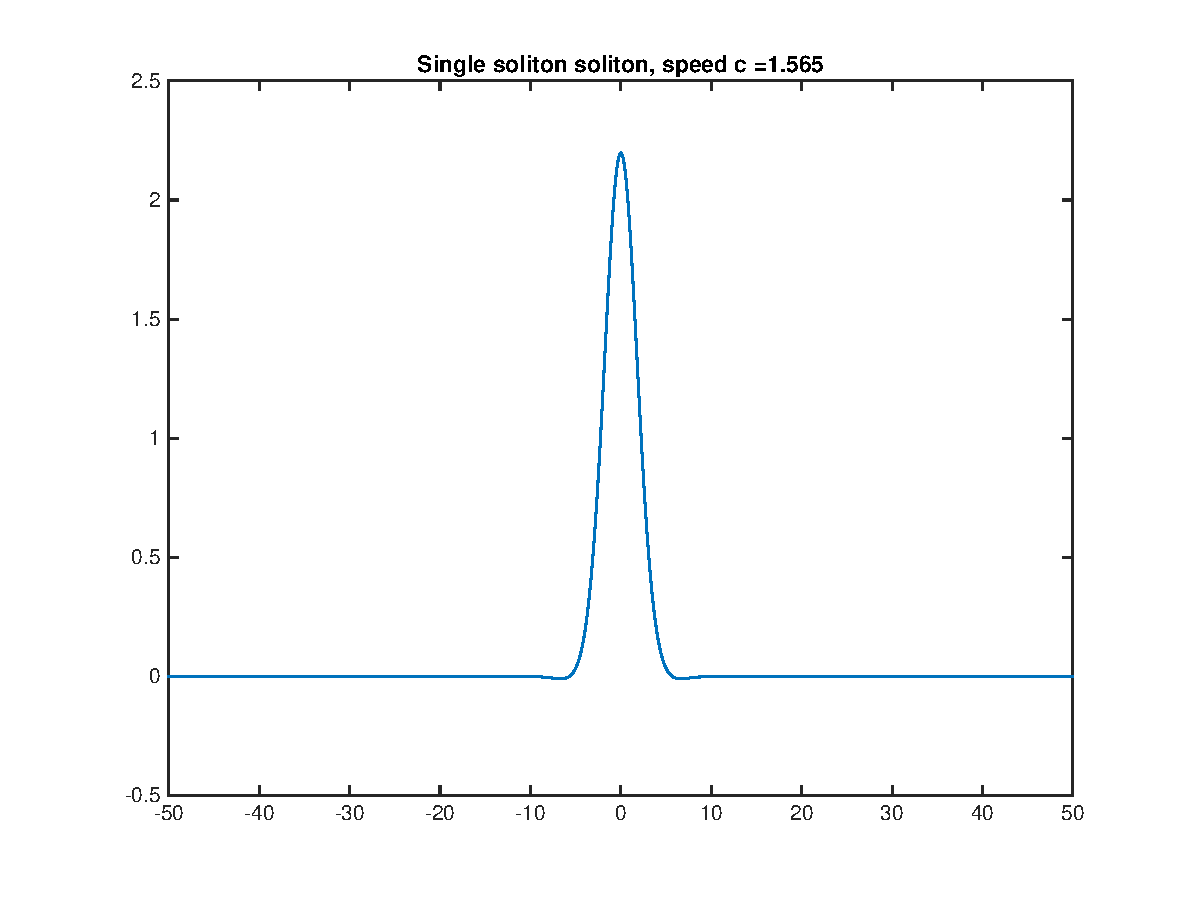
\includegraphics[width=8.5cm]{single.eps}
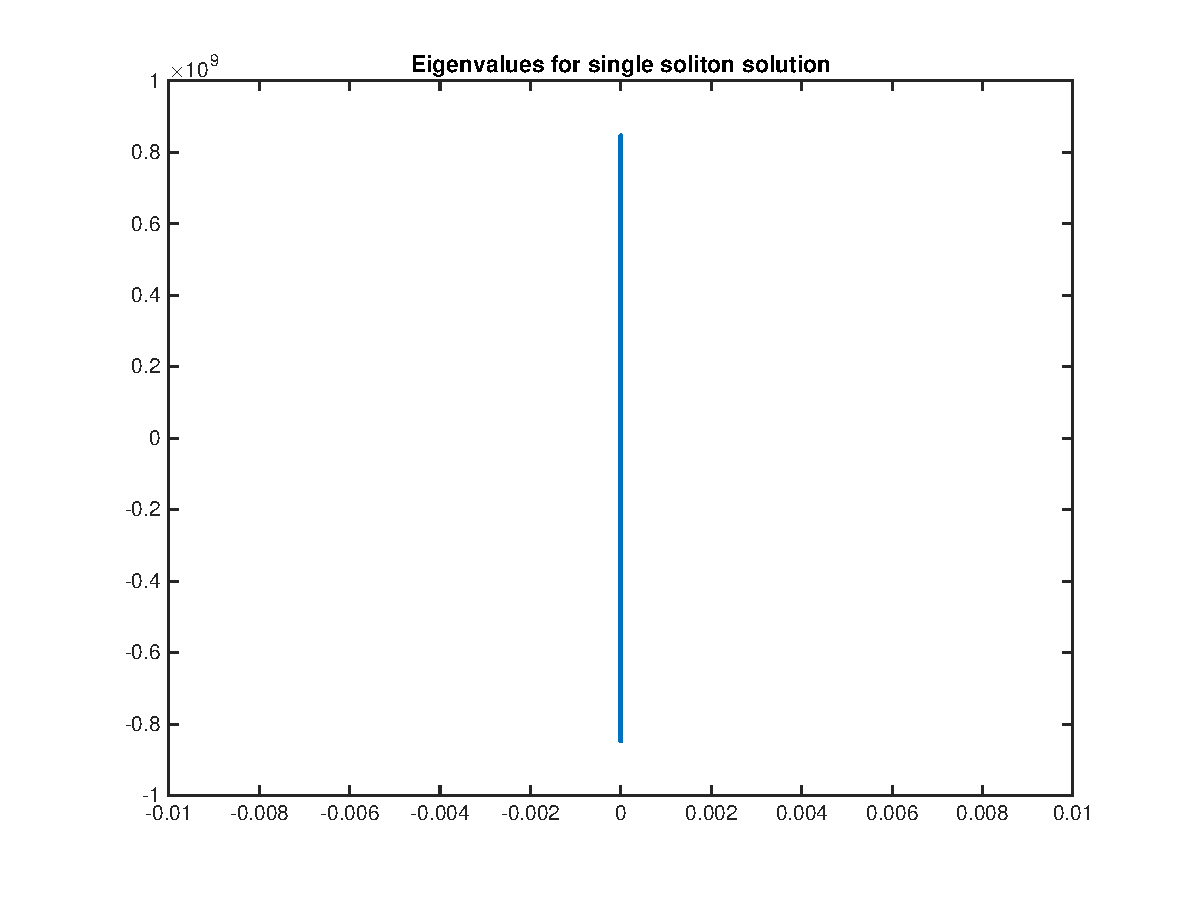
\includegraphics[width=8.5cm]{singleeig.eps}
\end{figure}

\item Double pulse joined at the first min/max and its eigenvalues. There are two eigenvalues on the real axis, which are symmetric about the origin. Zooming in, it does not look like they are complex conjugate pairs. Corresponding eigenfunctions also have no imaginary part, which supports the idea that these eigenvalues are real. Eigenfunctions are also plotted (plot title says ``real part'', which is all we have since eigenfunctions are real.)\\

Let $\lambda$ and $-\lambda$ be the two eigenvalues. (In this case, $\lambda = 0.0085$). Let $v(x)$ be the eigenfunction corresponding to $\lambda$. Then from the Matlab plots and data, the eigenfunction corresponding to $-\lambda$ is $v(-x)$, as expected. Note that in the Matlab plot, the eigenfunction corresponding to $-\lambda$ is actually $-v(-x)$, but this is okay since eigenfunctions only specified up to a scalar multiple. These eigenvalues and eigenfunctions are the same no matter which Matlab numerical eigenvalue method we use (i.e. using \textrm{nobalance} does not affect anything). We can also find the same eigenvalues and eigenfunctions using \textrm{eigs} centered anywhere except 0. From all this, I am convinced that these eigenvalues and eigenfunctions are correct.

\begin{figure}[H]
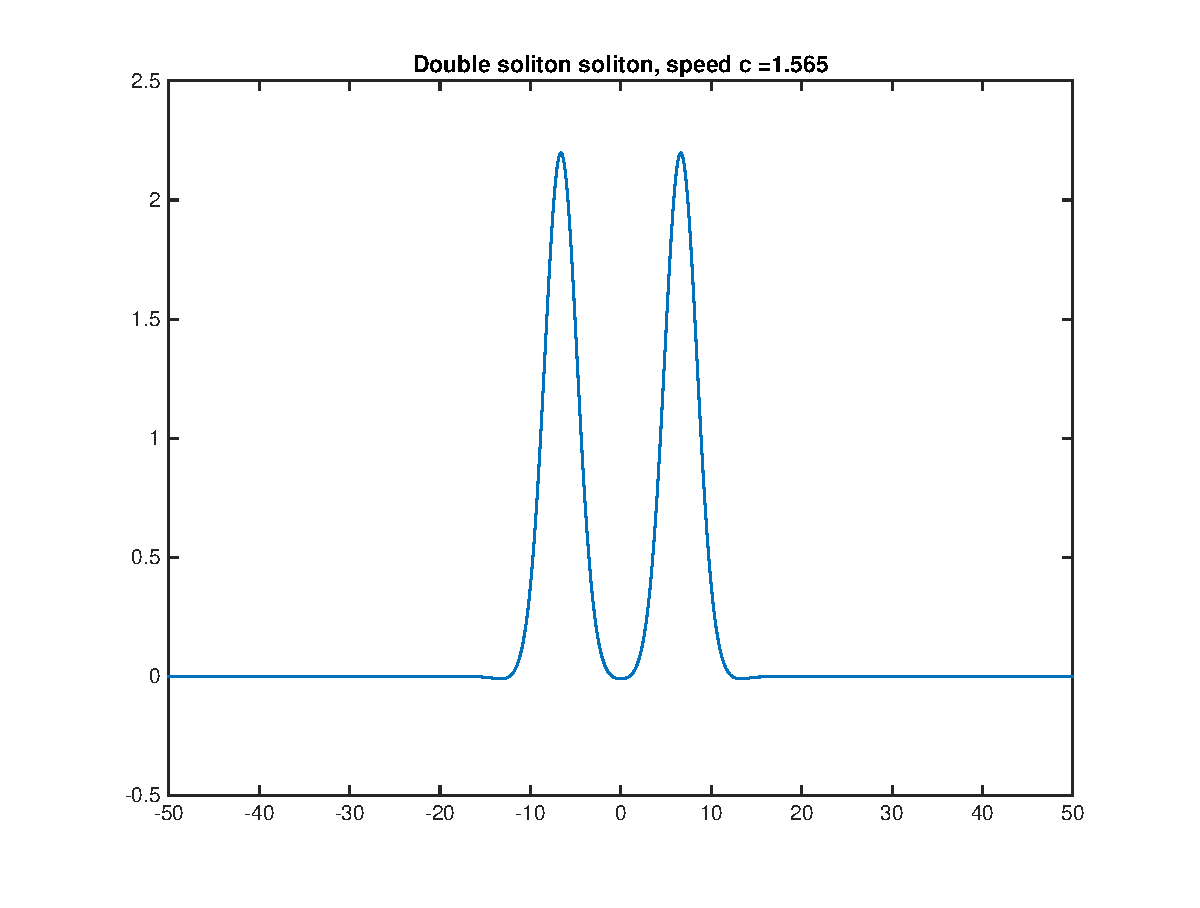
\includegraphics[width=8.5cm]{double1.eps}
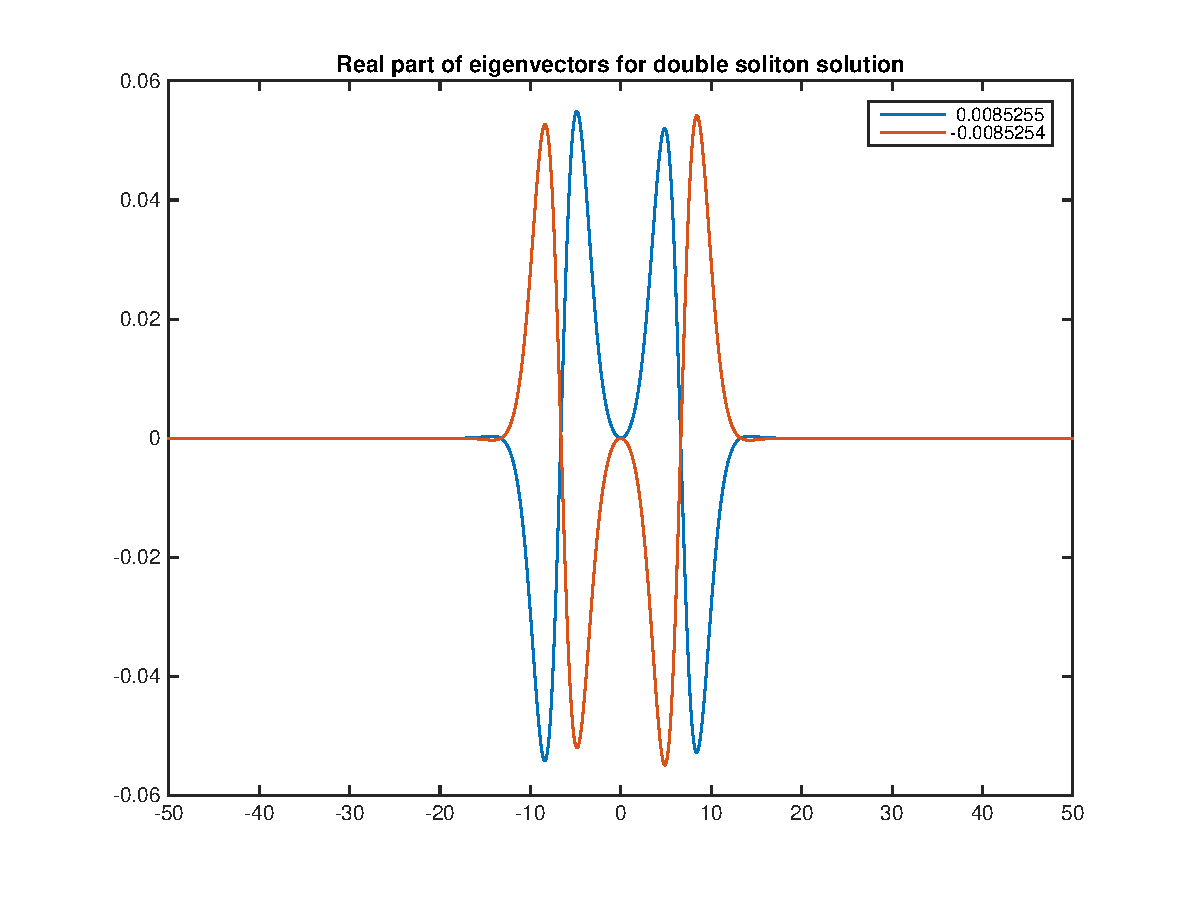
\includegraphics[width=8.5cm]{double1vec.eps}
\end{figure}

\begin{figure}[H]
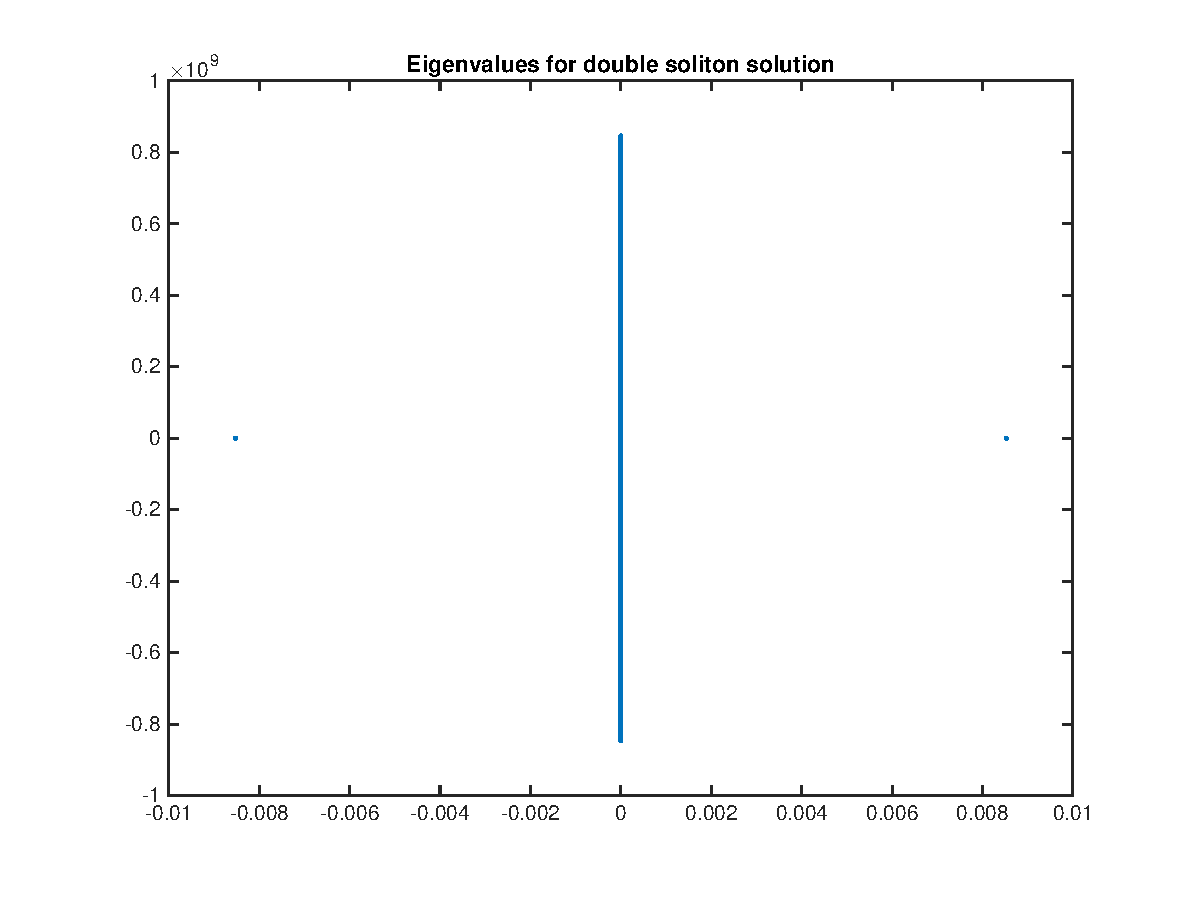
\includegraphics[width=8.5cm]{double1eig.eps}
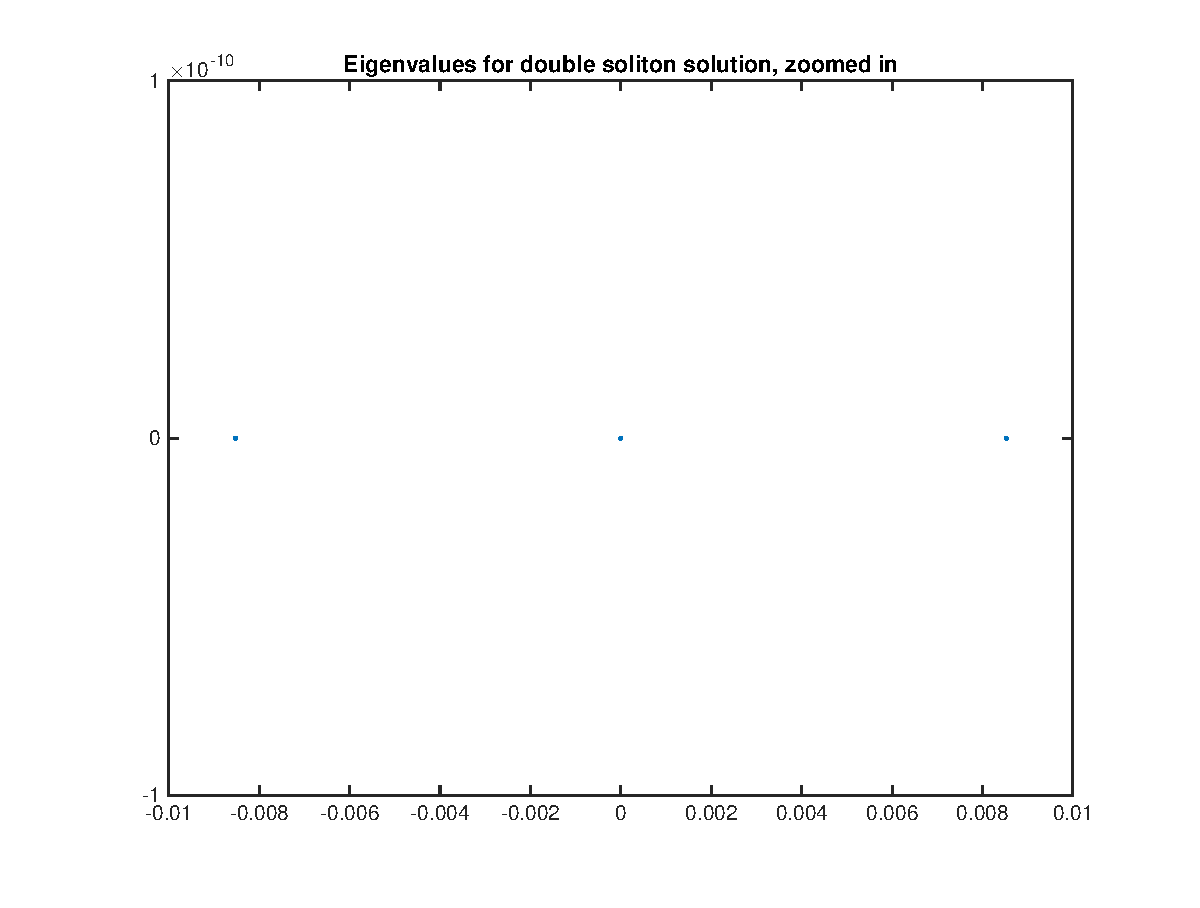
\includegraphics[width=8.5cm]{double1eigzoom.eps}
\end{figure}

\item Double pulse joined at the second min/max and its eigenvalues. Here we can zoom in and see that the eigenvalues are complex conjugate pairs located symmetrically about the real axis (i.e. quadruplet). Compared with the above double pulse, the eigenvalues are closer to the imaginary axis than the ones above. We also plot corresponding eigenfunctions to the quadruplet (absolute value, real part, and imaginary part).

\begin{figure}[H]
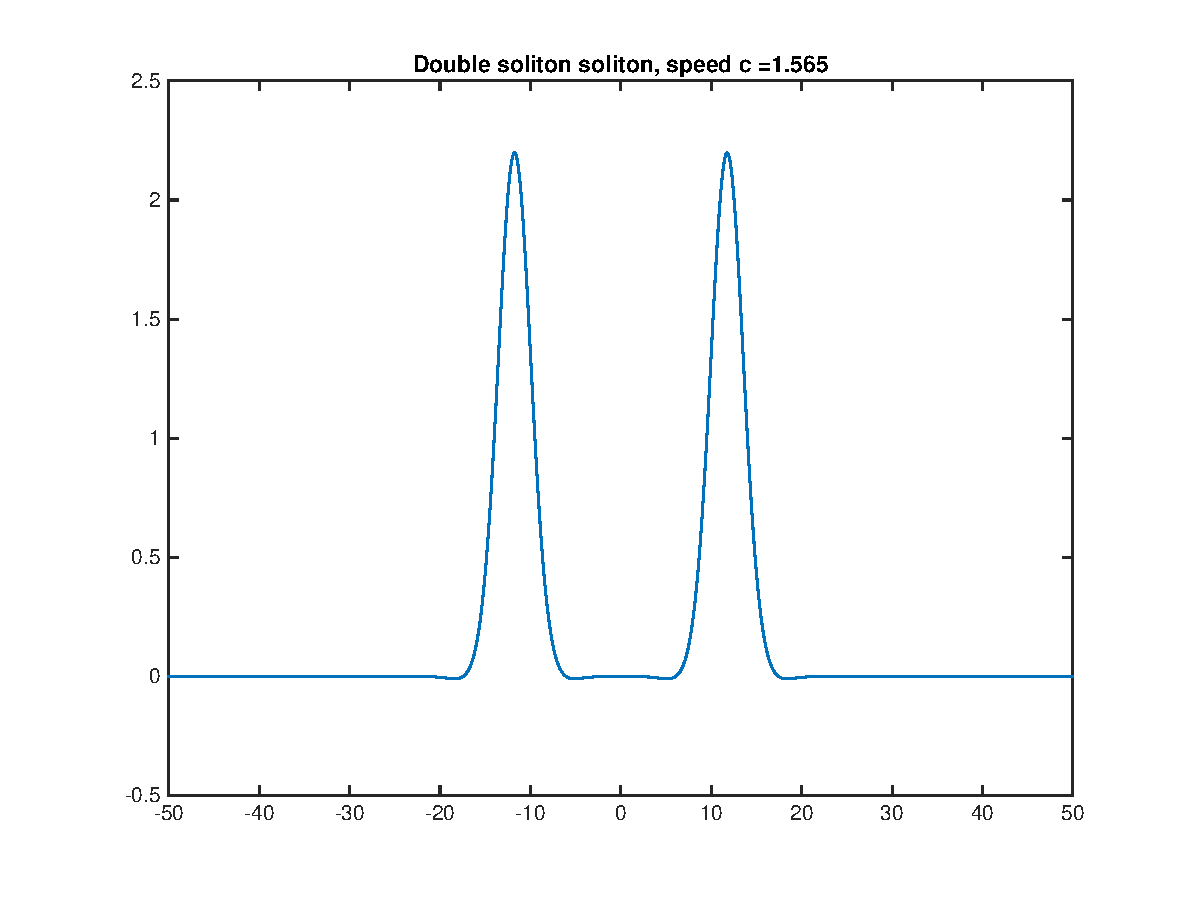
\includegraphics[width=8.5cm]{double2.eps}
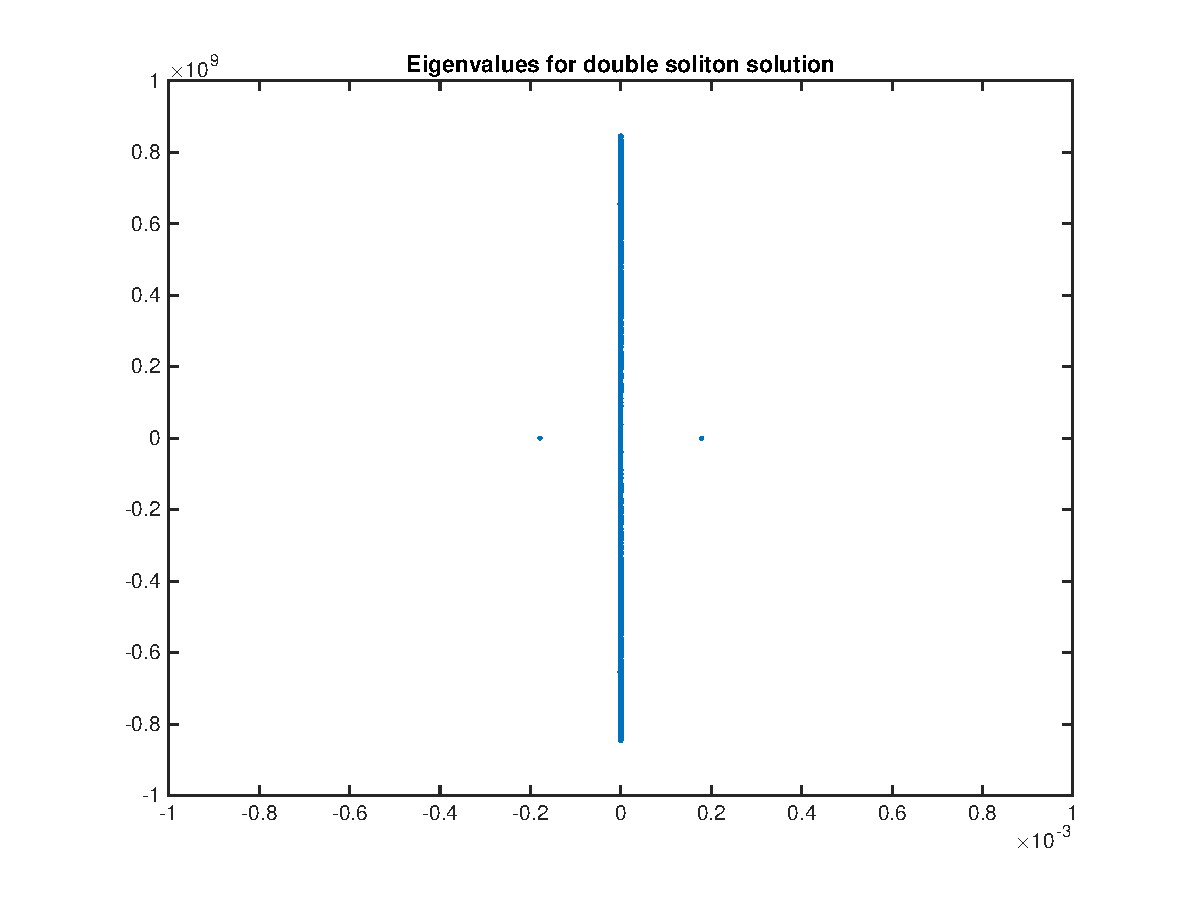
\includegraphics[width=8.5cm]{double2eig.eps}
\end{figure}

\begin{figure}[H]
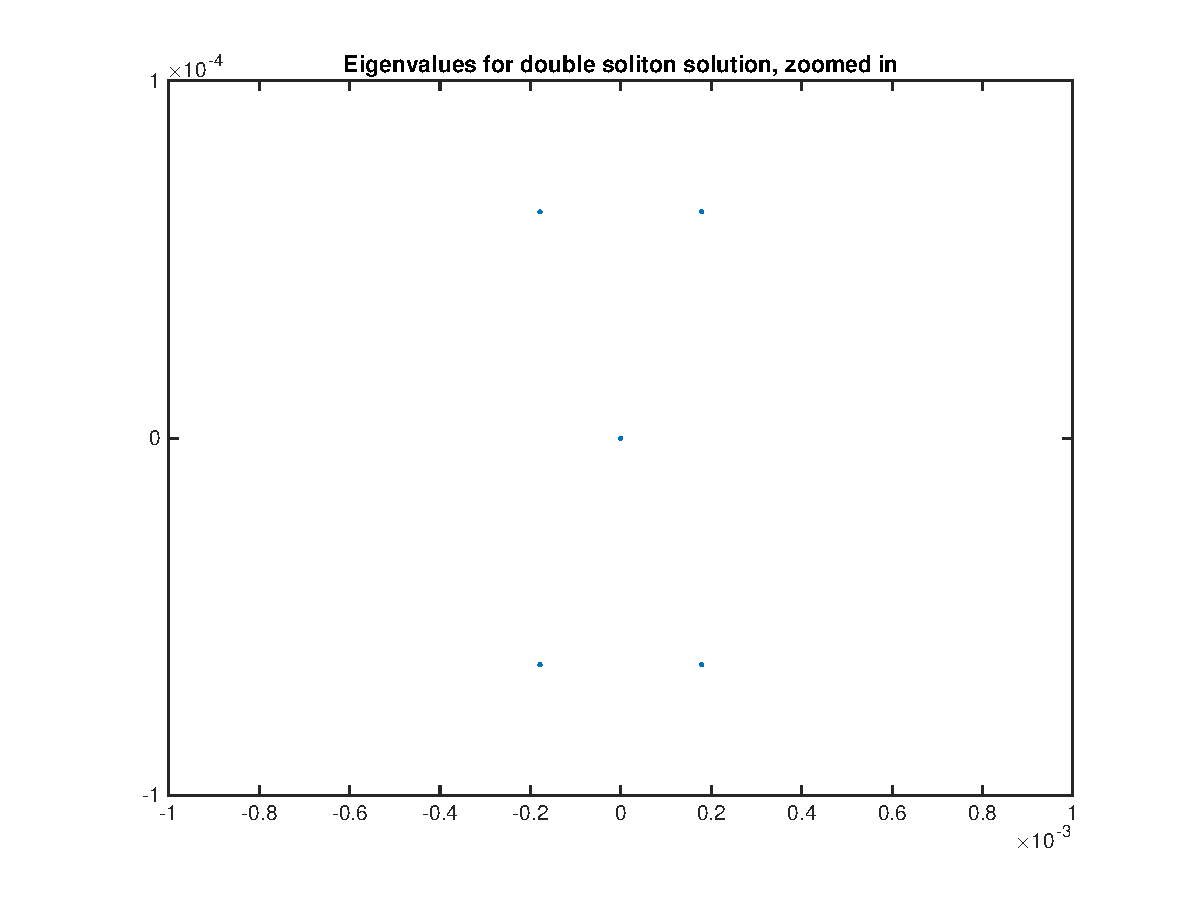
\includegraphics[width=8.5cm]{double2eigzoom.eps}
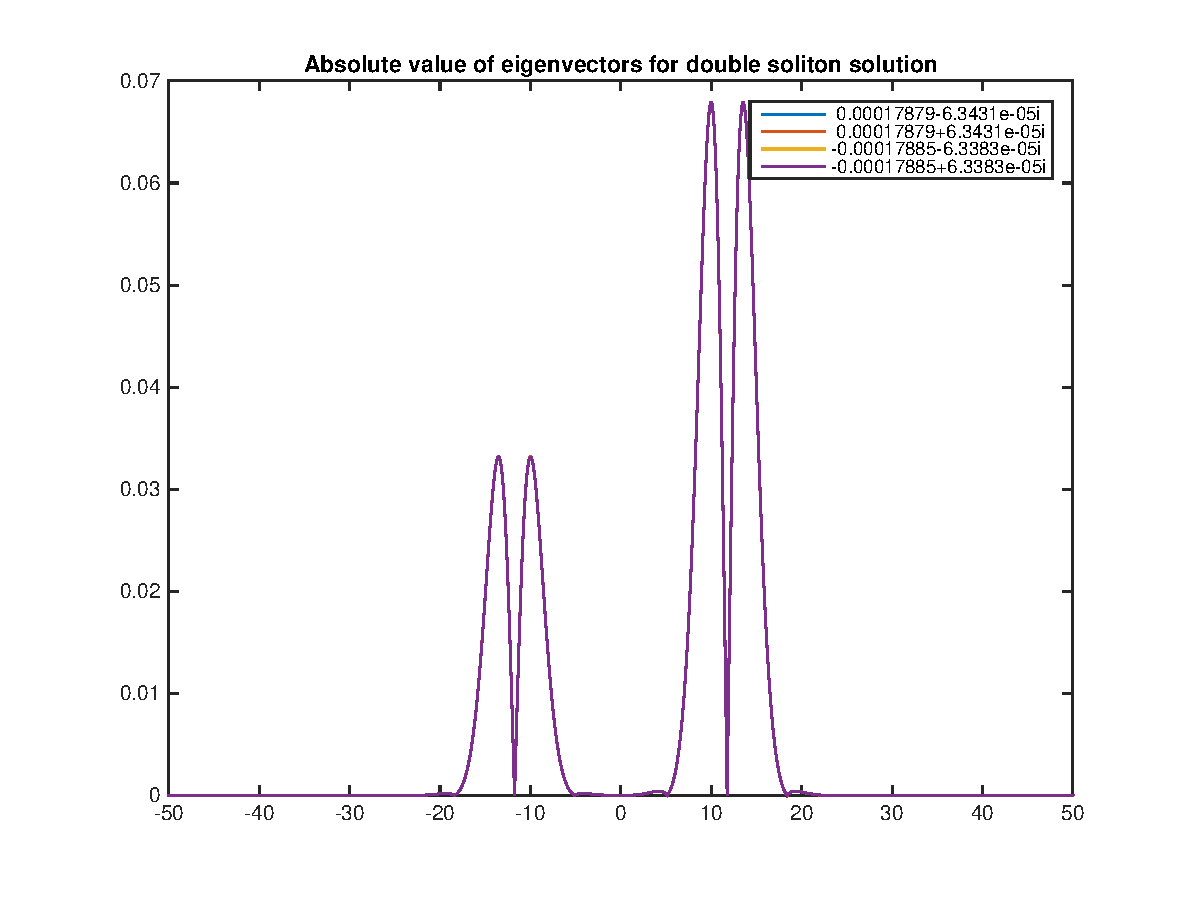
\includegraphics[width=8.5cm]{double2vecabs.eps}
\end{figure}

\begin{figure}[H]
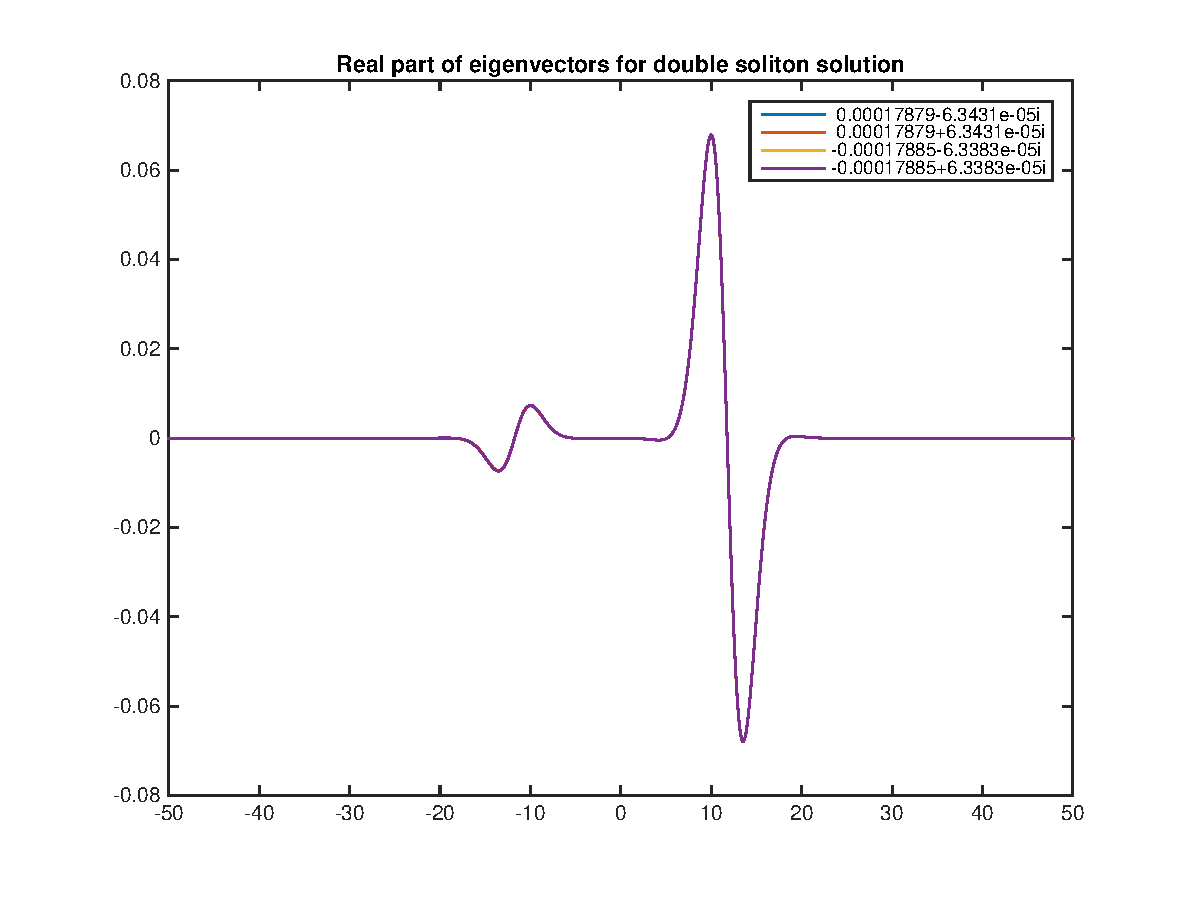
\includegraphics[width=8.5cm]{double2vecreal.eps}
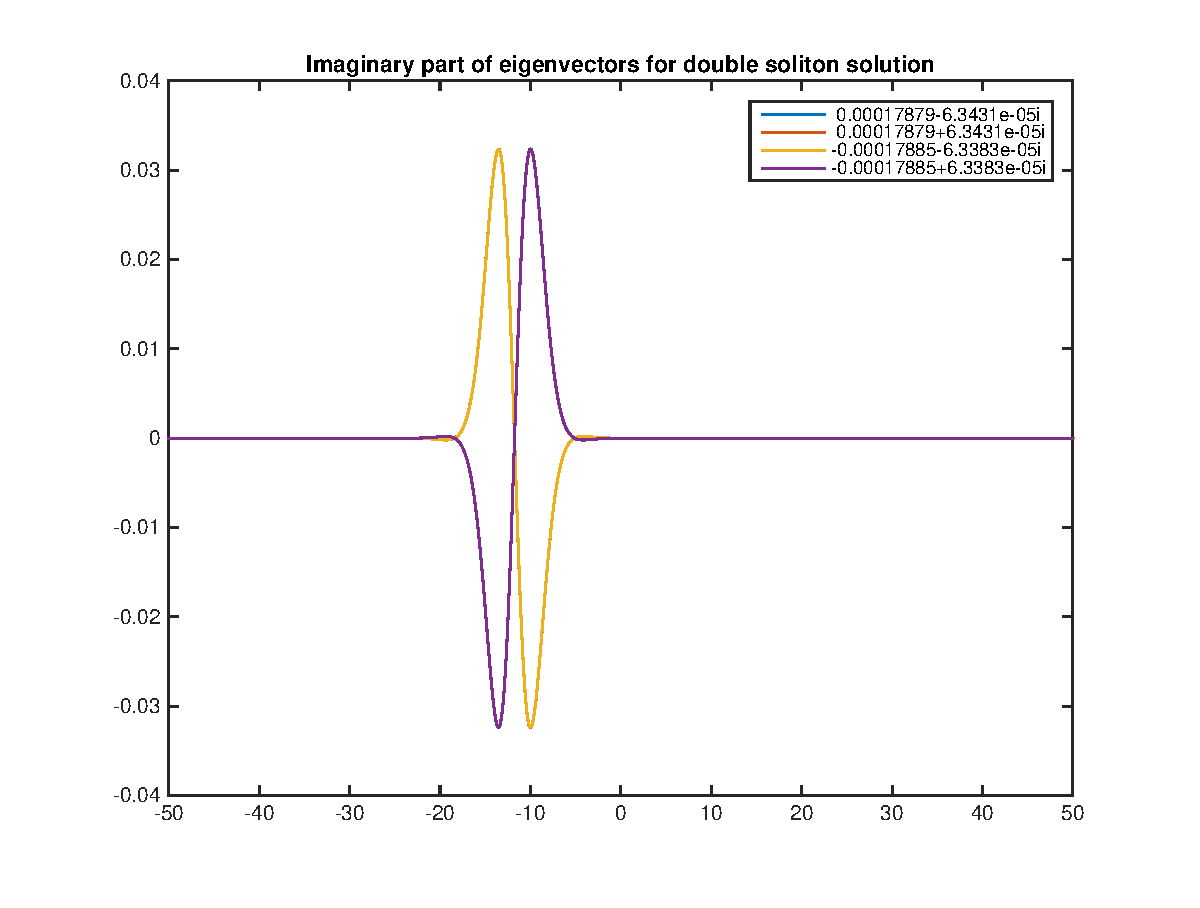
\includegraphics[width=8.5cm]{double2vecimag.eps}
\end{figure}

\item Double pulse joined at the third min/max and its eigenvalues. Here we can zoom in and see that the eigenvalues are complex conjugate pairs located symmetrically about the real axis. Eigenvalues are closer still to the imaginary axis; it seems reasonable that the eigenvalues get closer to the imaginary axis as the pulse separation increases, since as the pulses get further apart, they are more like two independent pulses. Eigenfunctions are plotted as above.

\begin{figure}[H]
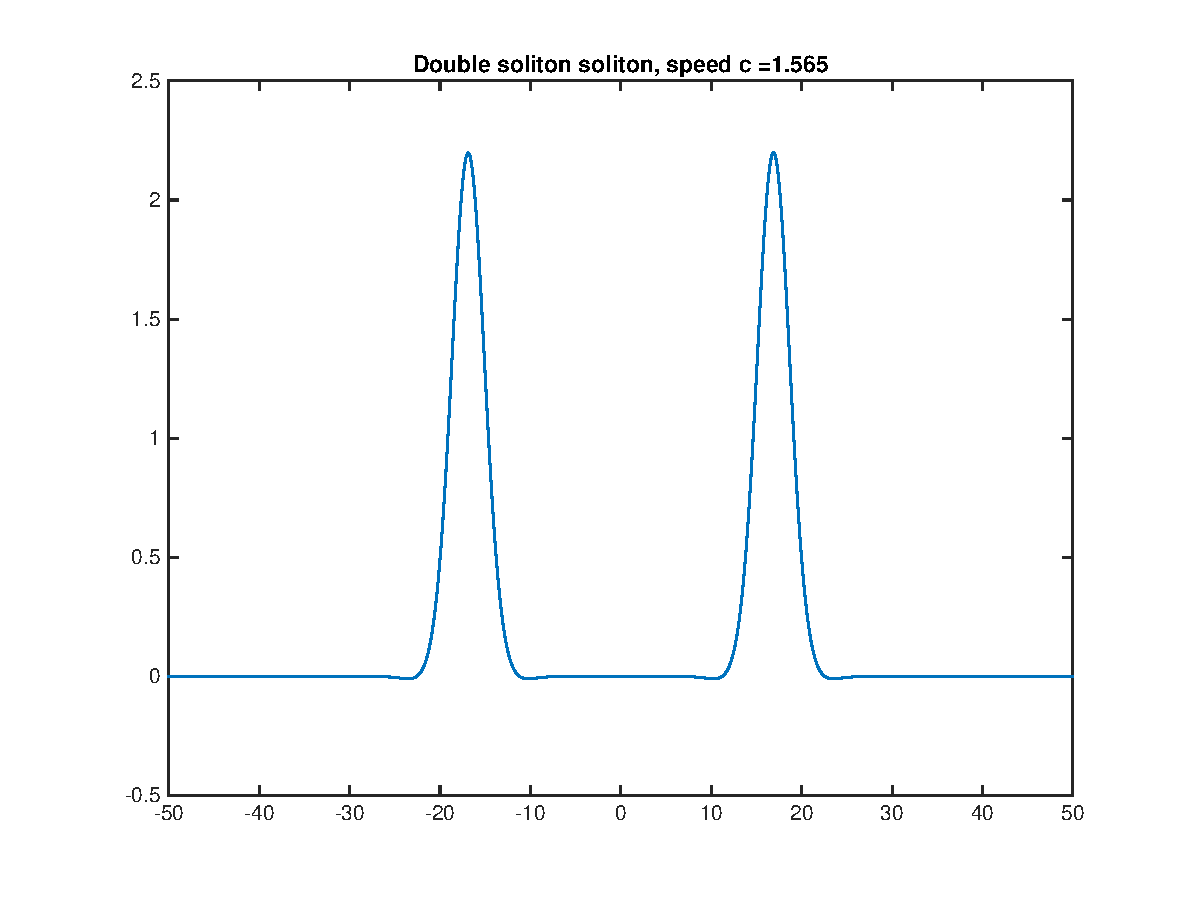
\includegraphics[width=8.5cm]{double3.eps}
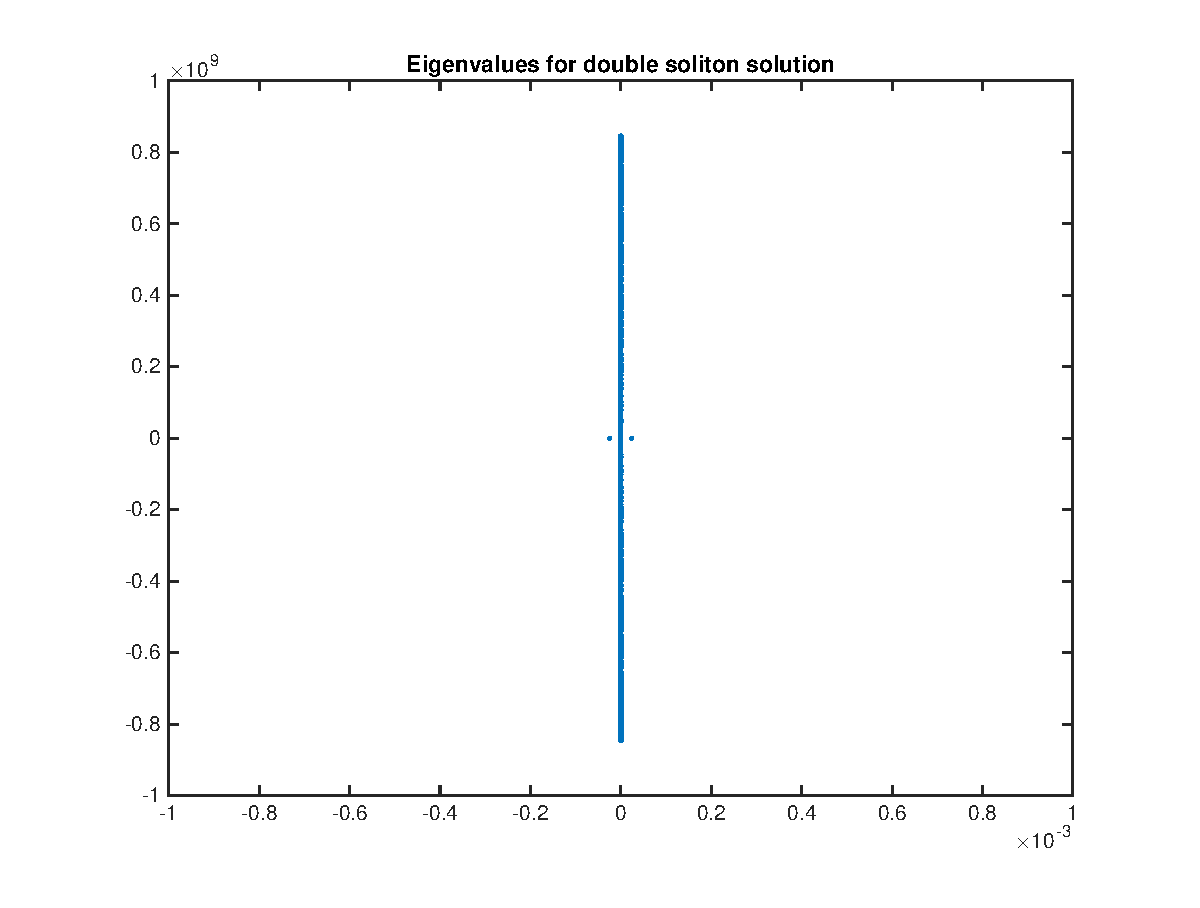
\includegraphics[width=8.5cm]{double3eig.eps}
\end{figure}

\begin{figure}[H]
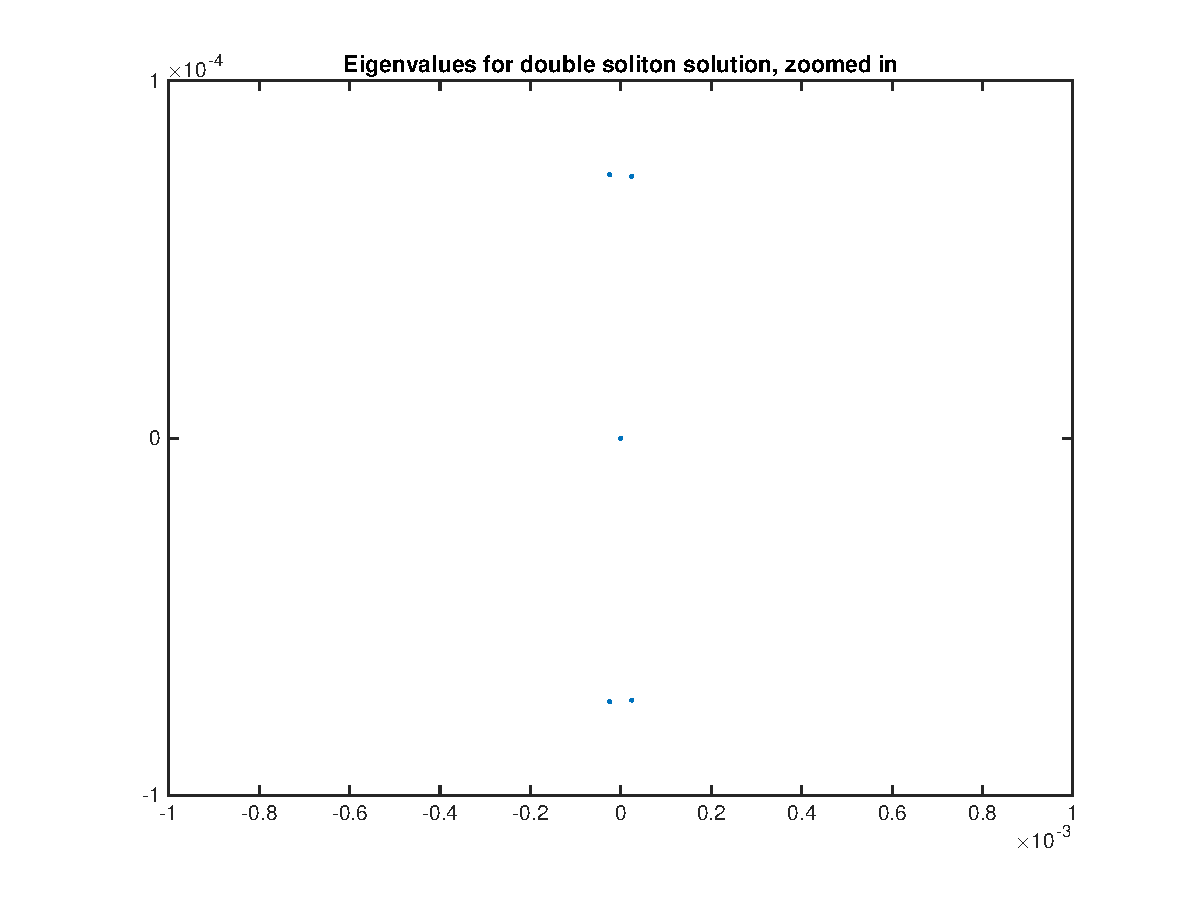
\includegraphics[width=8.5cm]{double3eigzoom.eps}
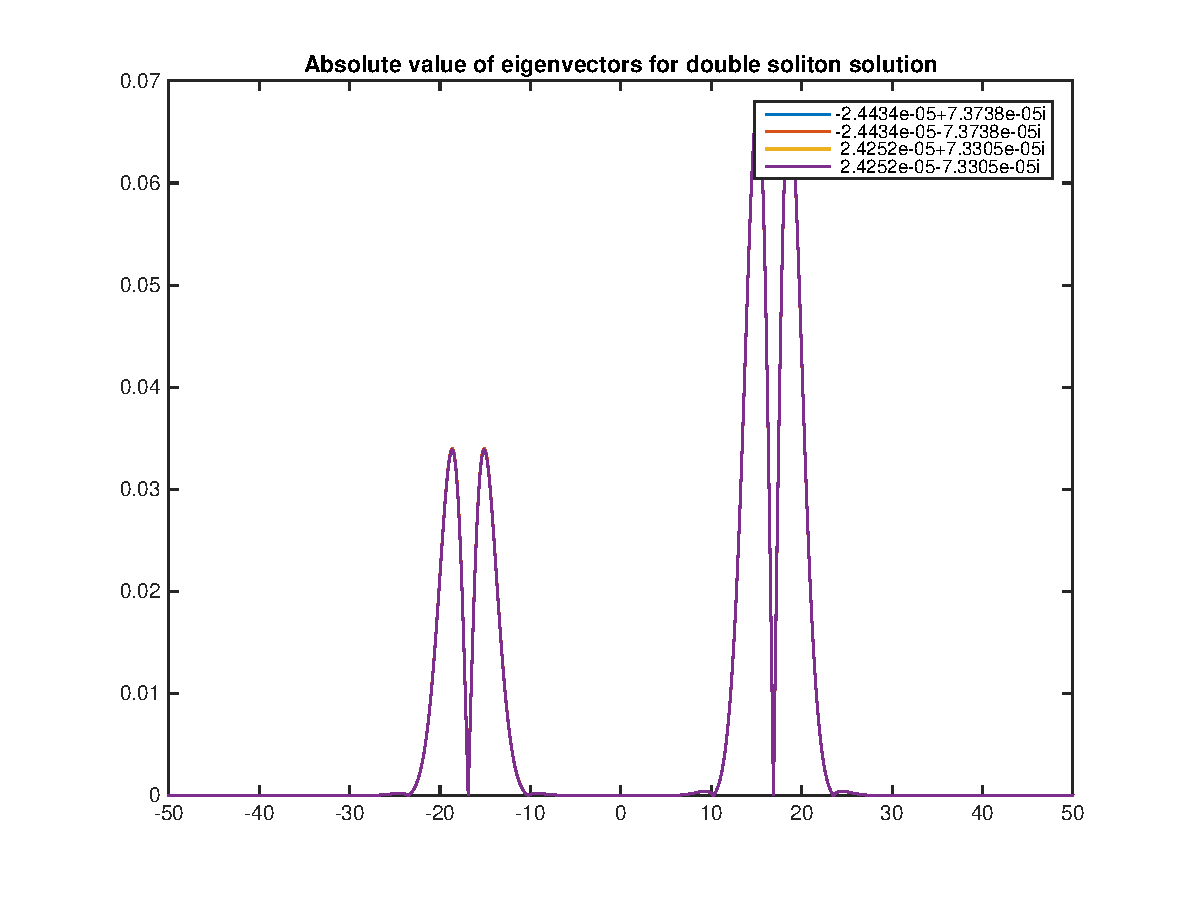
\includegraphics[width=8.5cm]{double3vecabs.eps}
\end{figure}

\begin{figure}[H]
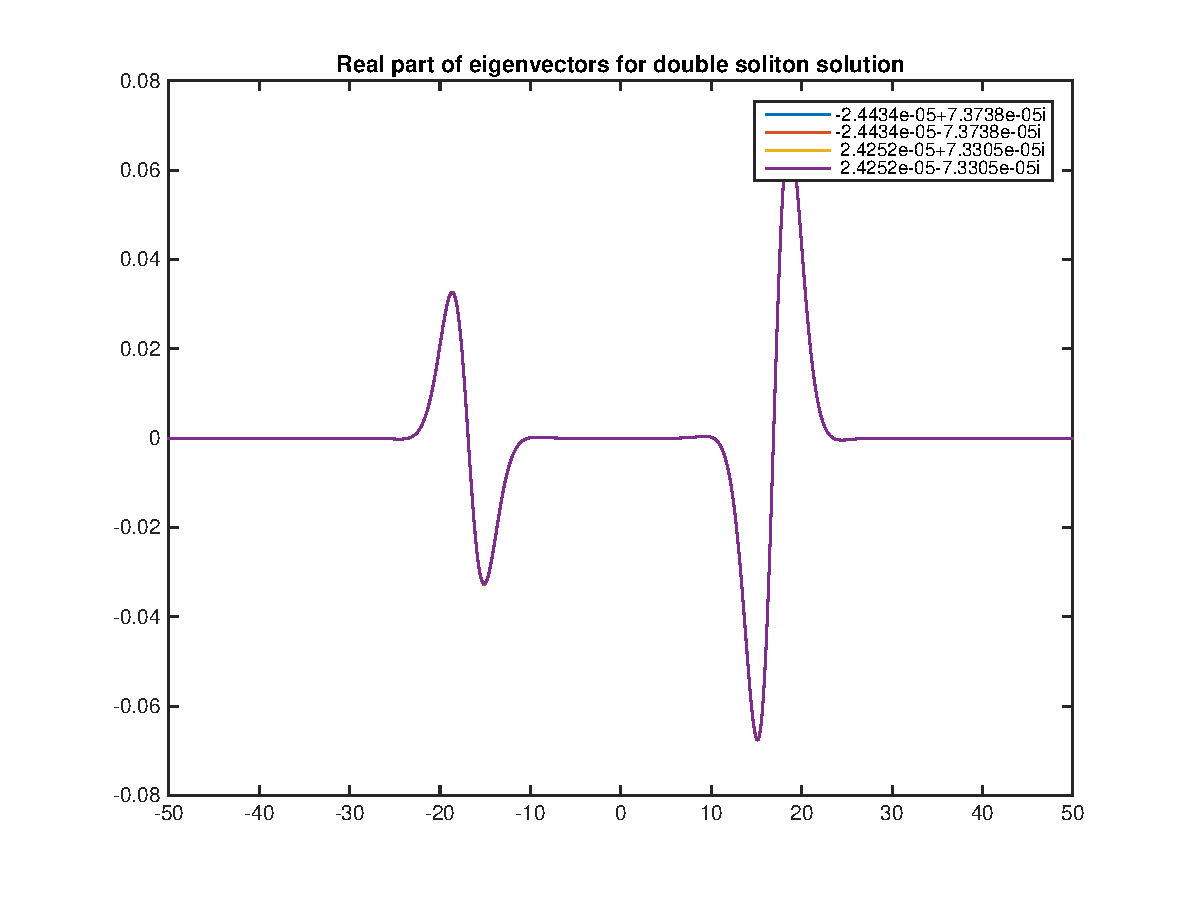
\includegraphics[width=8.5cm]{double3vecreal.eps}
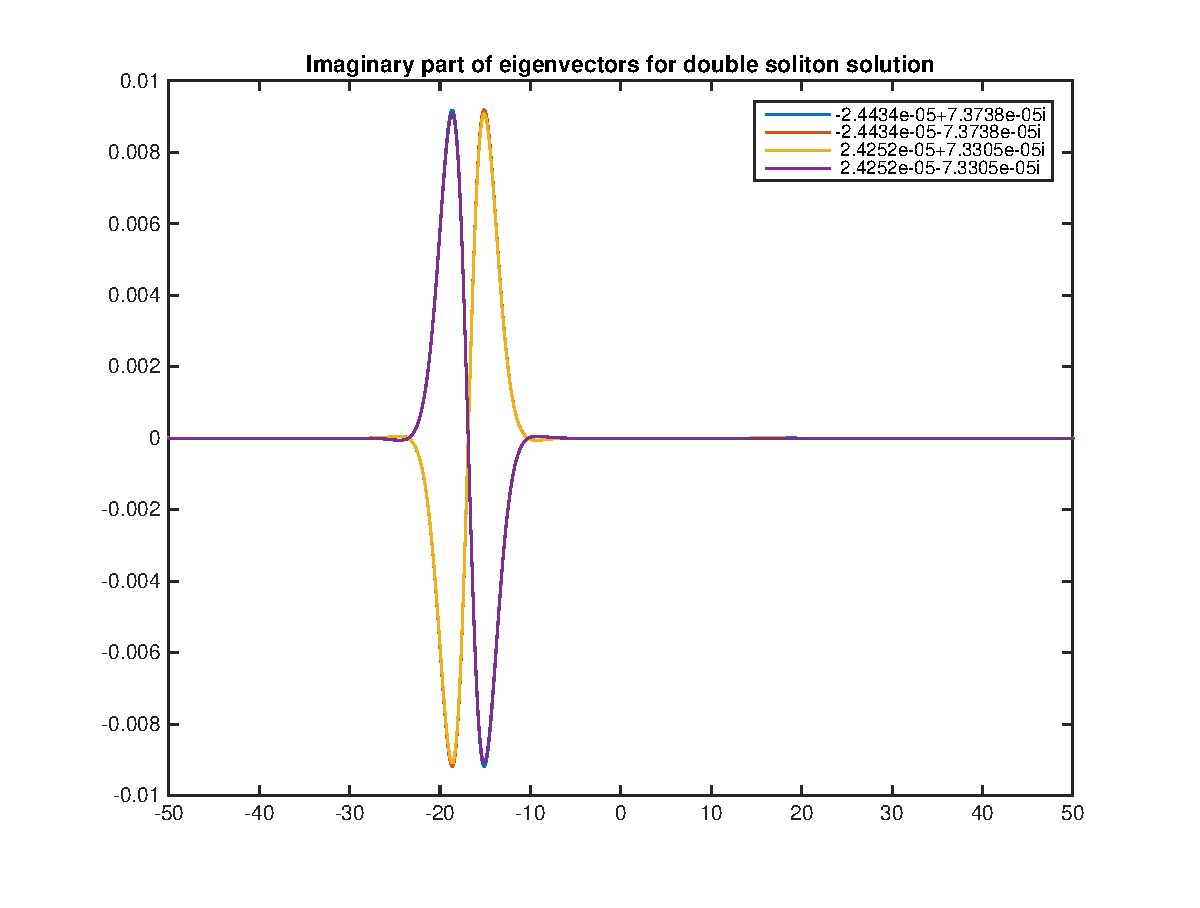
\includegraphics[width=8.5cm]{double3vecimag.eps}
\end{figure}

\item Double pulse joined at the fourth min/max and its eigenvalues. Here we can zoom in and see that the eigenvalues are complex conjugate pairs located symmetrically about the real axis. Eigenvalues are farther from the imaginary axis than the previous case, even though the pulses are farther apart, so maybe they do not always get closer. Eigenfunctions are plotted as above

\begin{figure}[H]
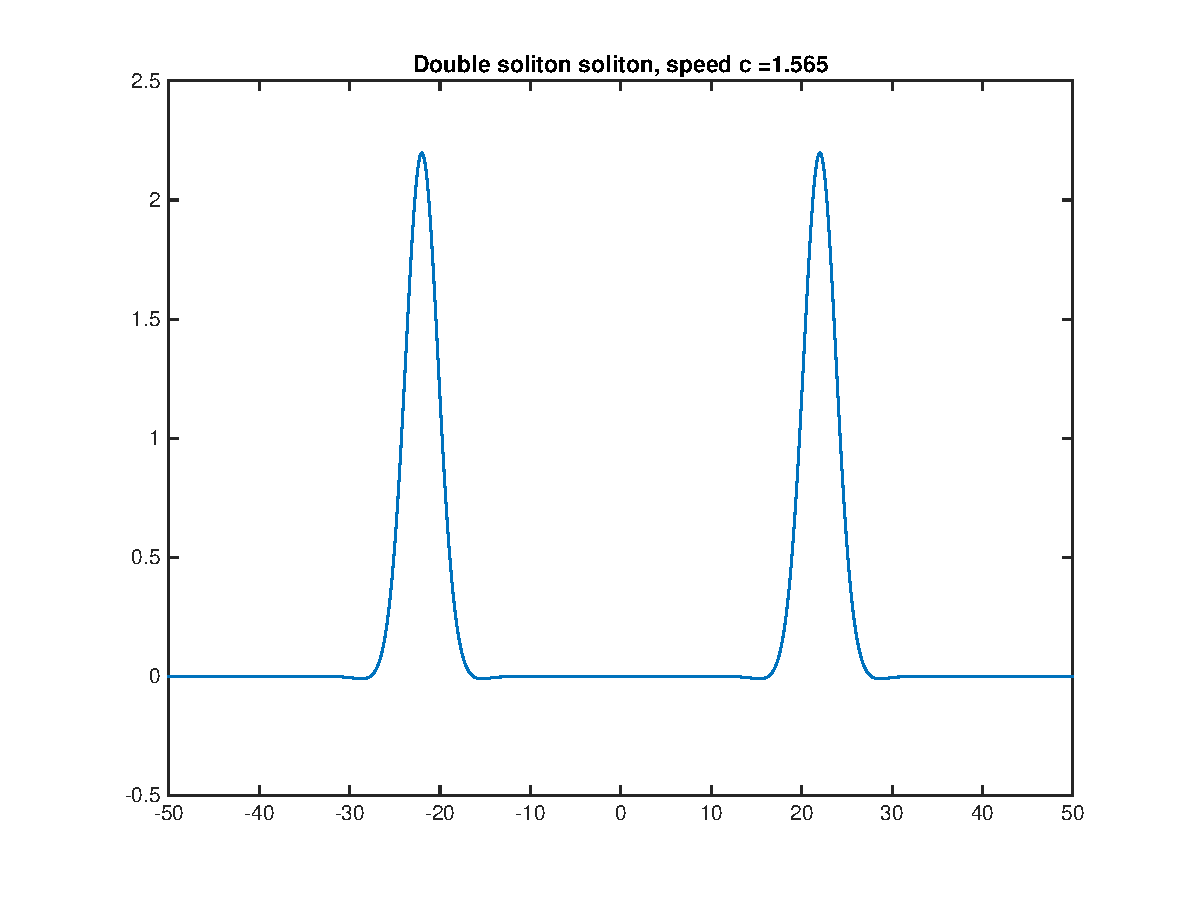
\includegraphics[width=8.5cm]{double4.eps}
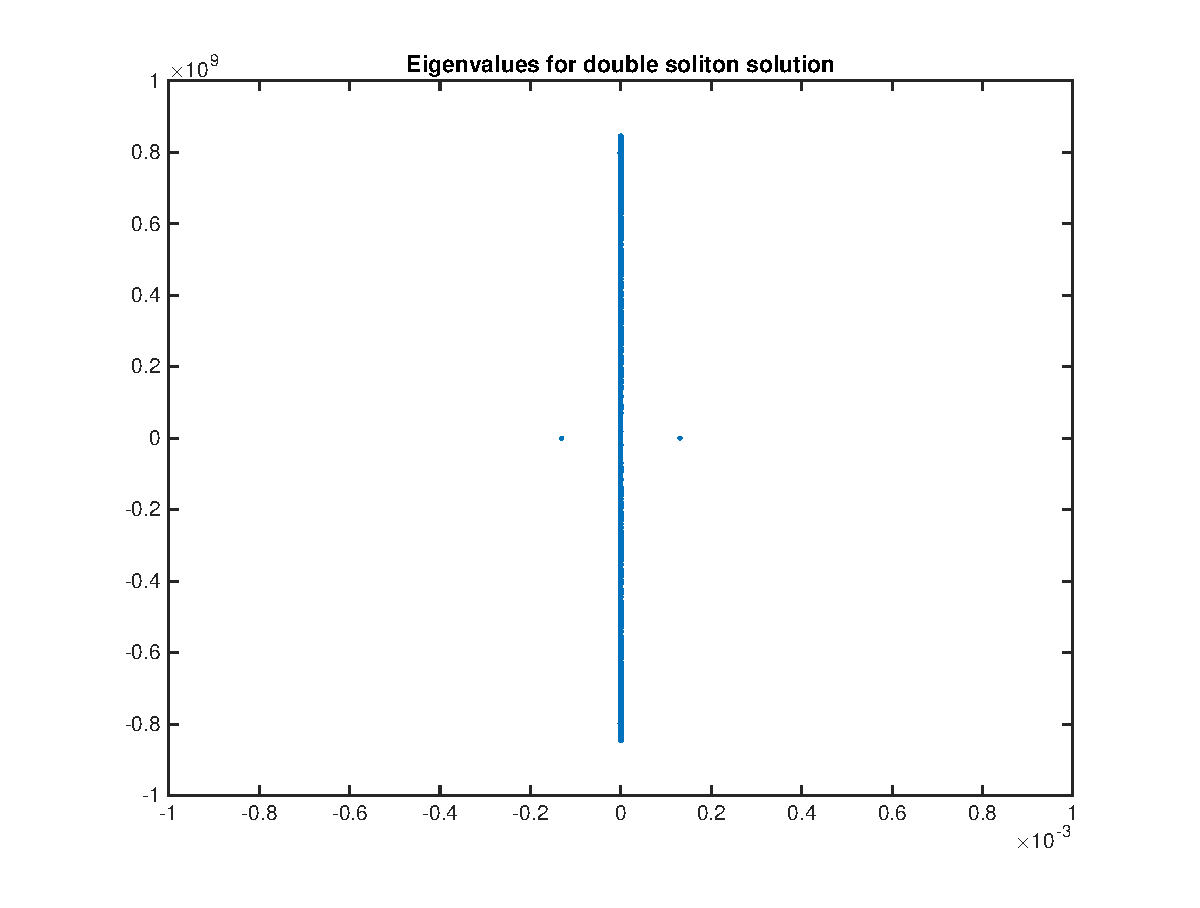
\includegraphics[width=8.5cm]{double4eig.eps}
\end{figure}

\begin{figure}[H]
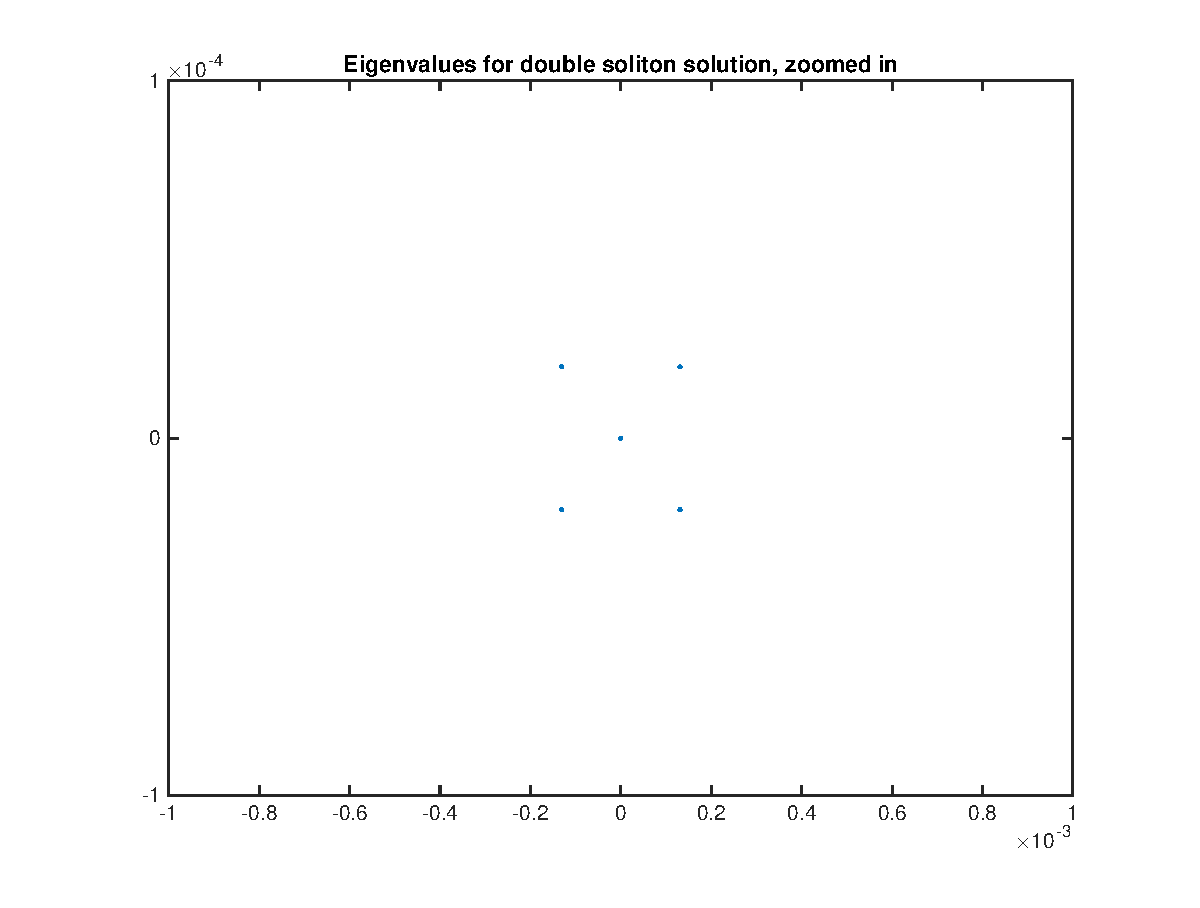
\includegraphics[width=8.5cm]{double4eigzoom.eps}
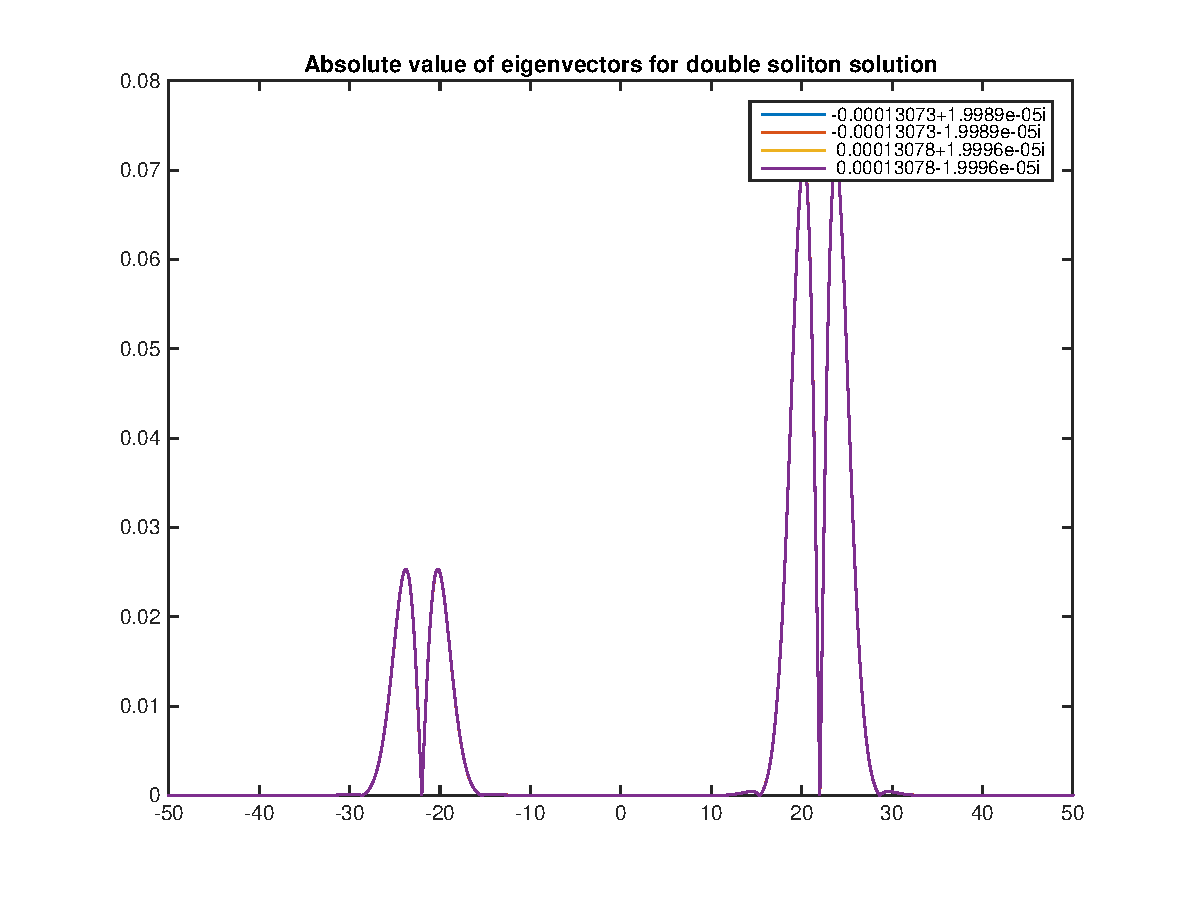
\includegraphics[width=8.5cm]{double4vecabs.eps}
\end{figure}

\begin{figure}[H]
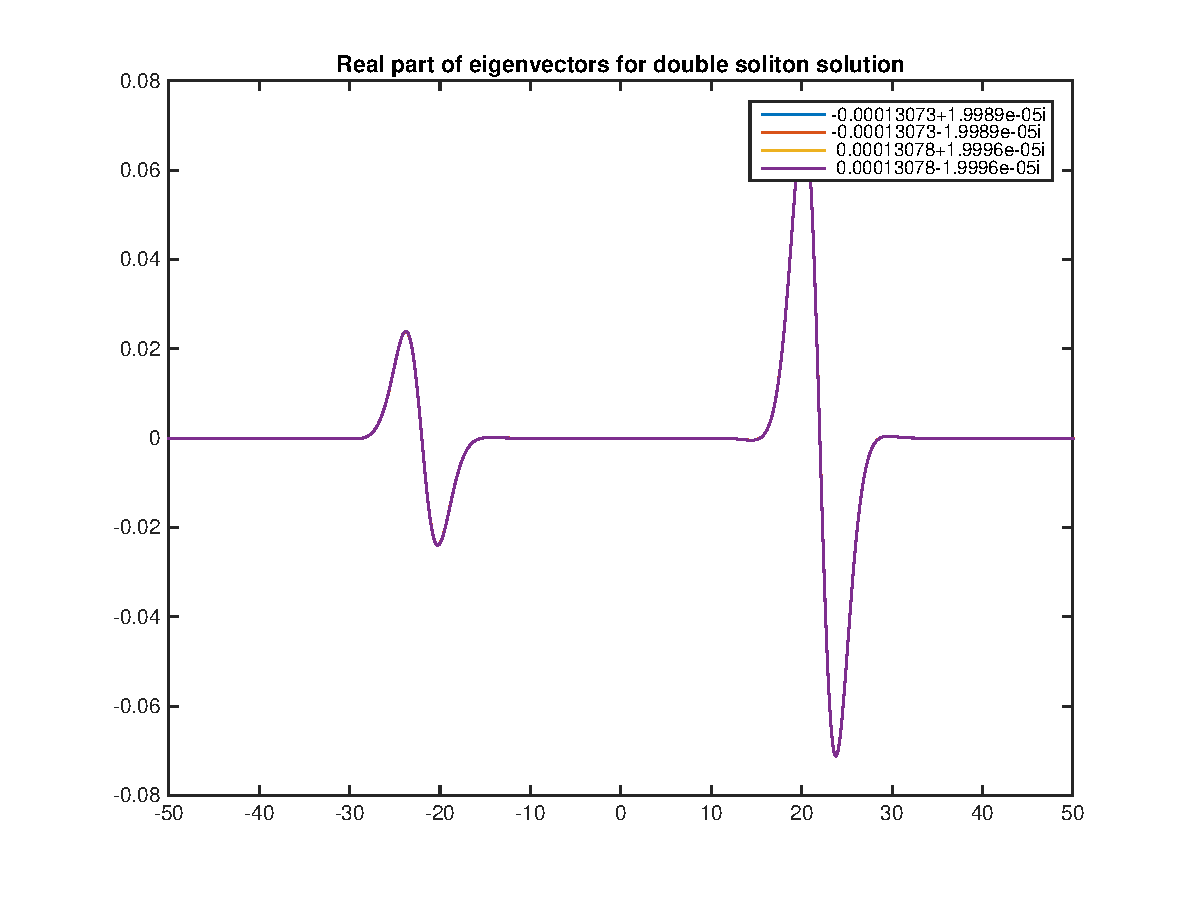
\includegraphics[width=8.5cm]{double4vecreal.eps}
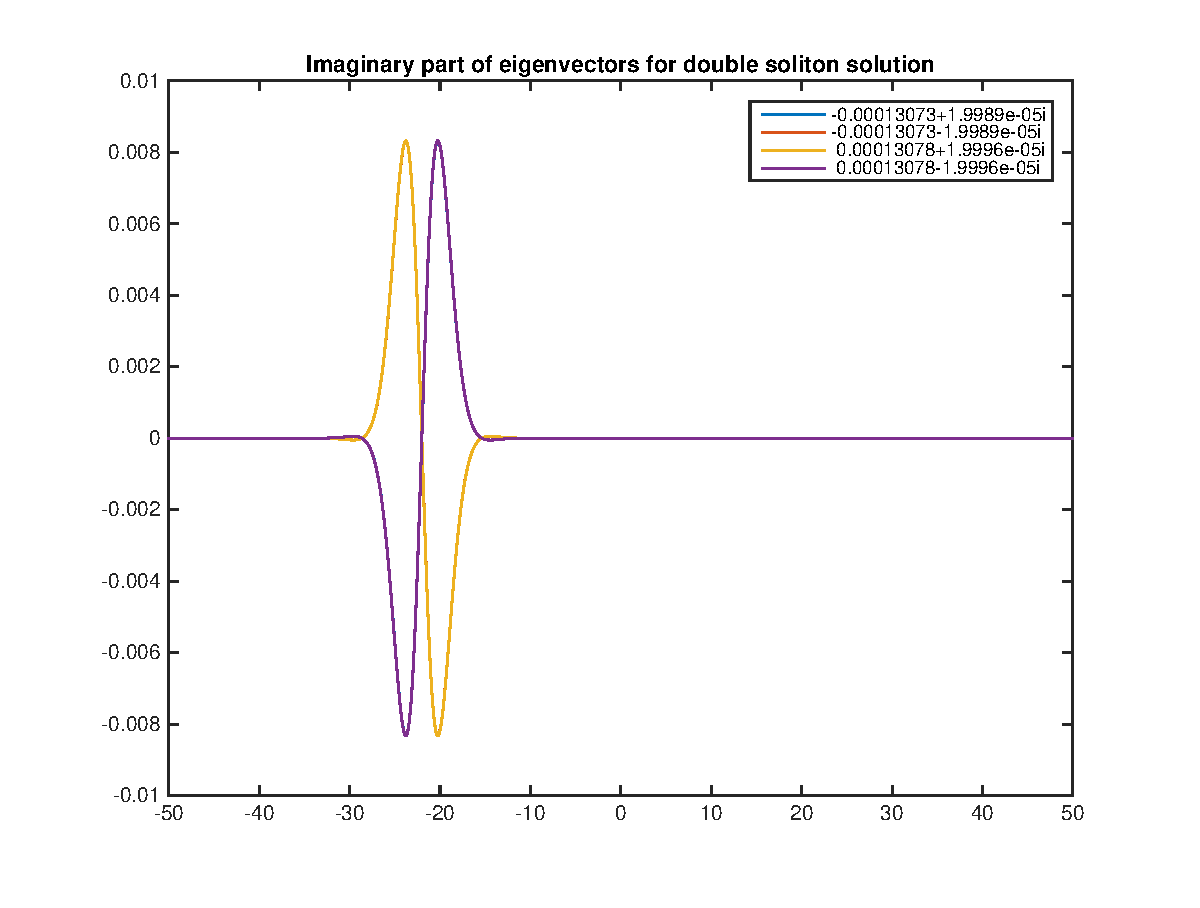
\includegraphics[width=8.5cm]{double4vecimag.eps}
\end{figure}

\end{enumerate}

I am not convinced that the double pulse for min/max 2-4 is correct. The quadruplet of eigenvalues we get are not of the form $\lambda, 
\bar{\lambda}, -\lambda, -\bar{\lambda}$; the real part of the negative eigenvalues is close, but not identical to the negative of the real part of the positive eigenvalues. They do come in complex conjugate pairs, which is good. Furthermore, if $\lambda$ is the eigenvalue in the first quadrant of the complex plane with eigenfunction $v(x)$, if we manually try $-\lambda$ and $v(-x)$, we get an approximate solution to the eigenvalue problem. Finally, if we use Matlab's \textrm{eigs}, we get different eigenvalues (with nonnegative real part) depending on what we choose as the ``center'' for \textrm{eigs}. That being said, I do believe that there are eigenvalues near this location, and the eigenfunctions look approximately like the ones I have.

\section*{7 January, 2017}
\subsection*{Extend domain}
Reran code from above, extending domain of half-wave to $[0,100]$ (2000 grid points) and full wave to $[-100, 100]$. In other words, more ``zero-padding'' around our solitary wave. Everything else was the same. In this case, we are using \textrm{eigs} instead of \textrm{eig} since the latter is too slow with this many grid points. The continuation method gives us a single puse for $c = 1.5647$, very close to the $c = 1.5650$ used above. We then construct double pulses as we did above.
\begin{enumerate}
	\item Pulses joined at first min/max
	\begin{figure}[H]
	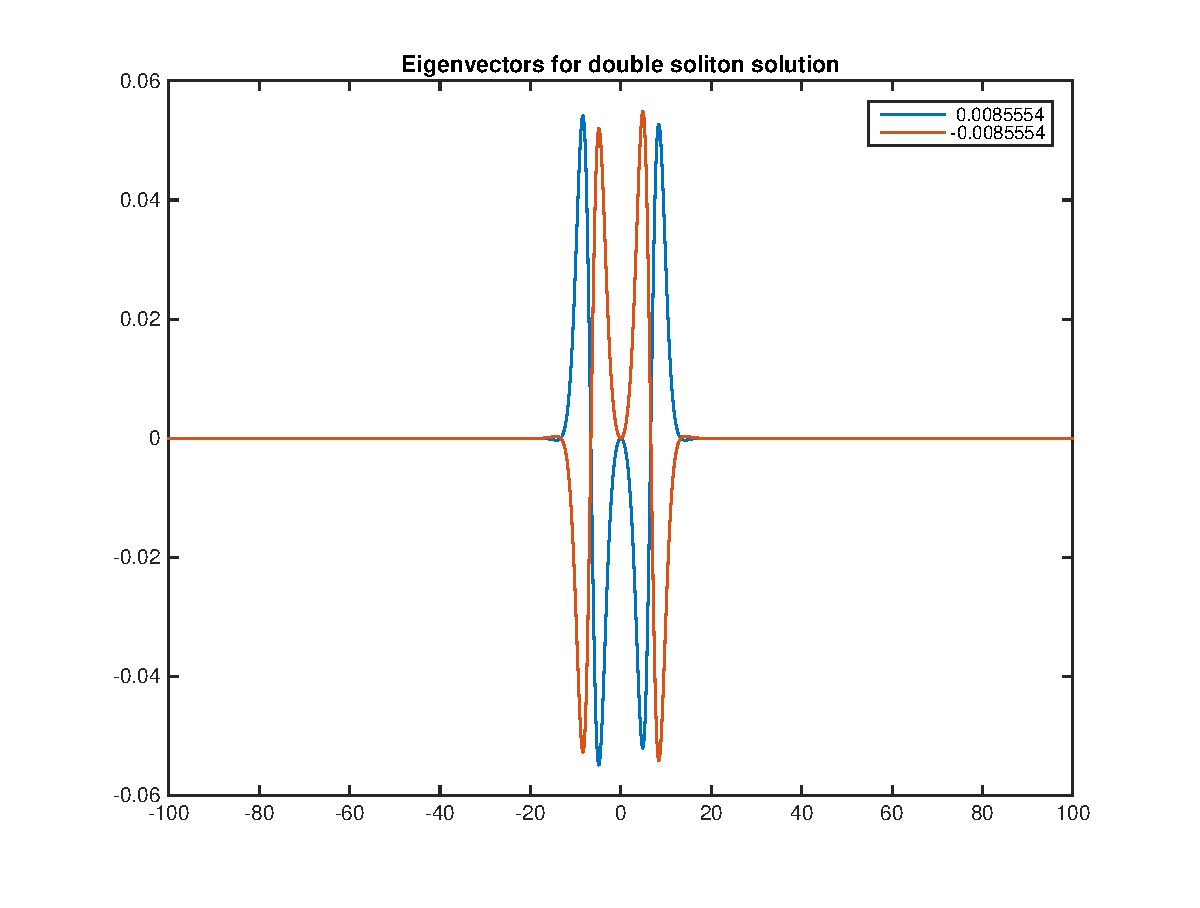
\includegraphics[width=8.5cm]{double1vec_100.eps}
	\end{figure}
	These look almost identical to the ones we got above with the smaller domain. Eigenvalues are $0.0085554, -0.0085554$, which are negatives of each other and almost identital to those above, with the difference due to the slightly different value of $c$.

	\item Pulses joined at later min/max (2-3)\\
	We have the same problem as above. We can find eigenvalues/eigenfunctions with \textrm{eigs}, but the values differ depending on what we use as the center for \textrm{eig}.
	
\end{enumerate}

\end{document}

